\chapter{Artifactory}
Om de verschillende applicaties die ontwikkeld worden met elkaar te laten communiceren, hebben we een "Common Library" ontwikkeld. Deze library bevat verschillende interfaces die door elke applicatie gebruikt kunnen worden.
Deze library moeten we beschikbaar stellen in een repository voor de verschillende applicaties. Dit hebben we gerealiseerd door gebruikt te maken van Artifactory.

\section{Container configuratie}
Net zoals Sonarqube vereist het opzetten van Artifactory weinig configuratie binnen docker. Een verschil met de andere tools is echter wel dat de huidige versie van Artifactory niet beschikbaar is op docker hub. Hiervoor hebben we handmatig het commando uitgevoerd om de docker image binnen te halen vanuit de JFrog (ontwikkelaar van Artifactory) repository.
\newline
Tevens moeten we de poort configureren waarop Artifactory bereikbaar is. Standaard is dit poort 8081, echter was deze poort reeds in gebruikt door Jira. We hebben ervoor gekozen om Artifactory beschikbaar te maken op poort 8082.

\begin{figure}[H]
	\centering
	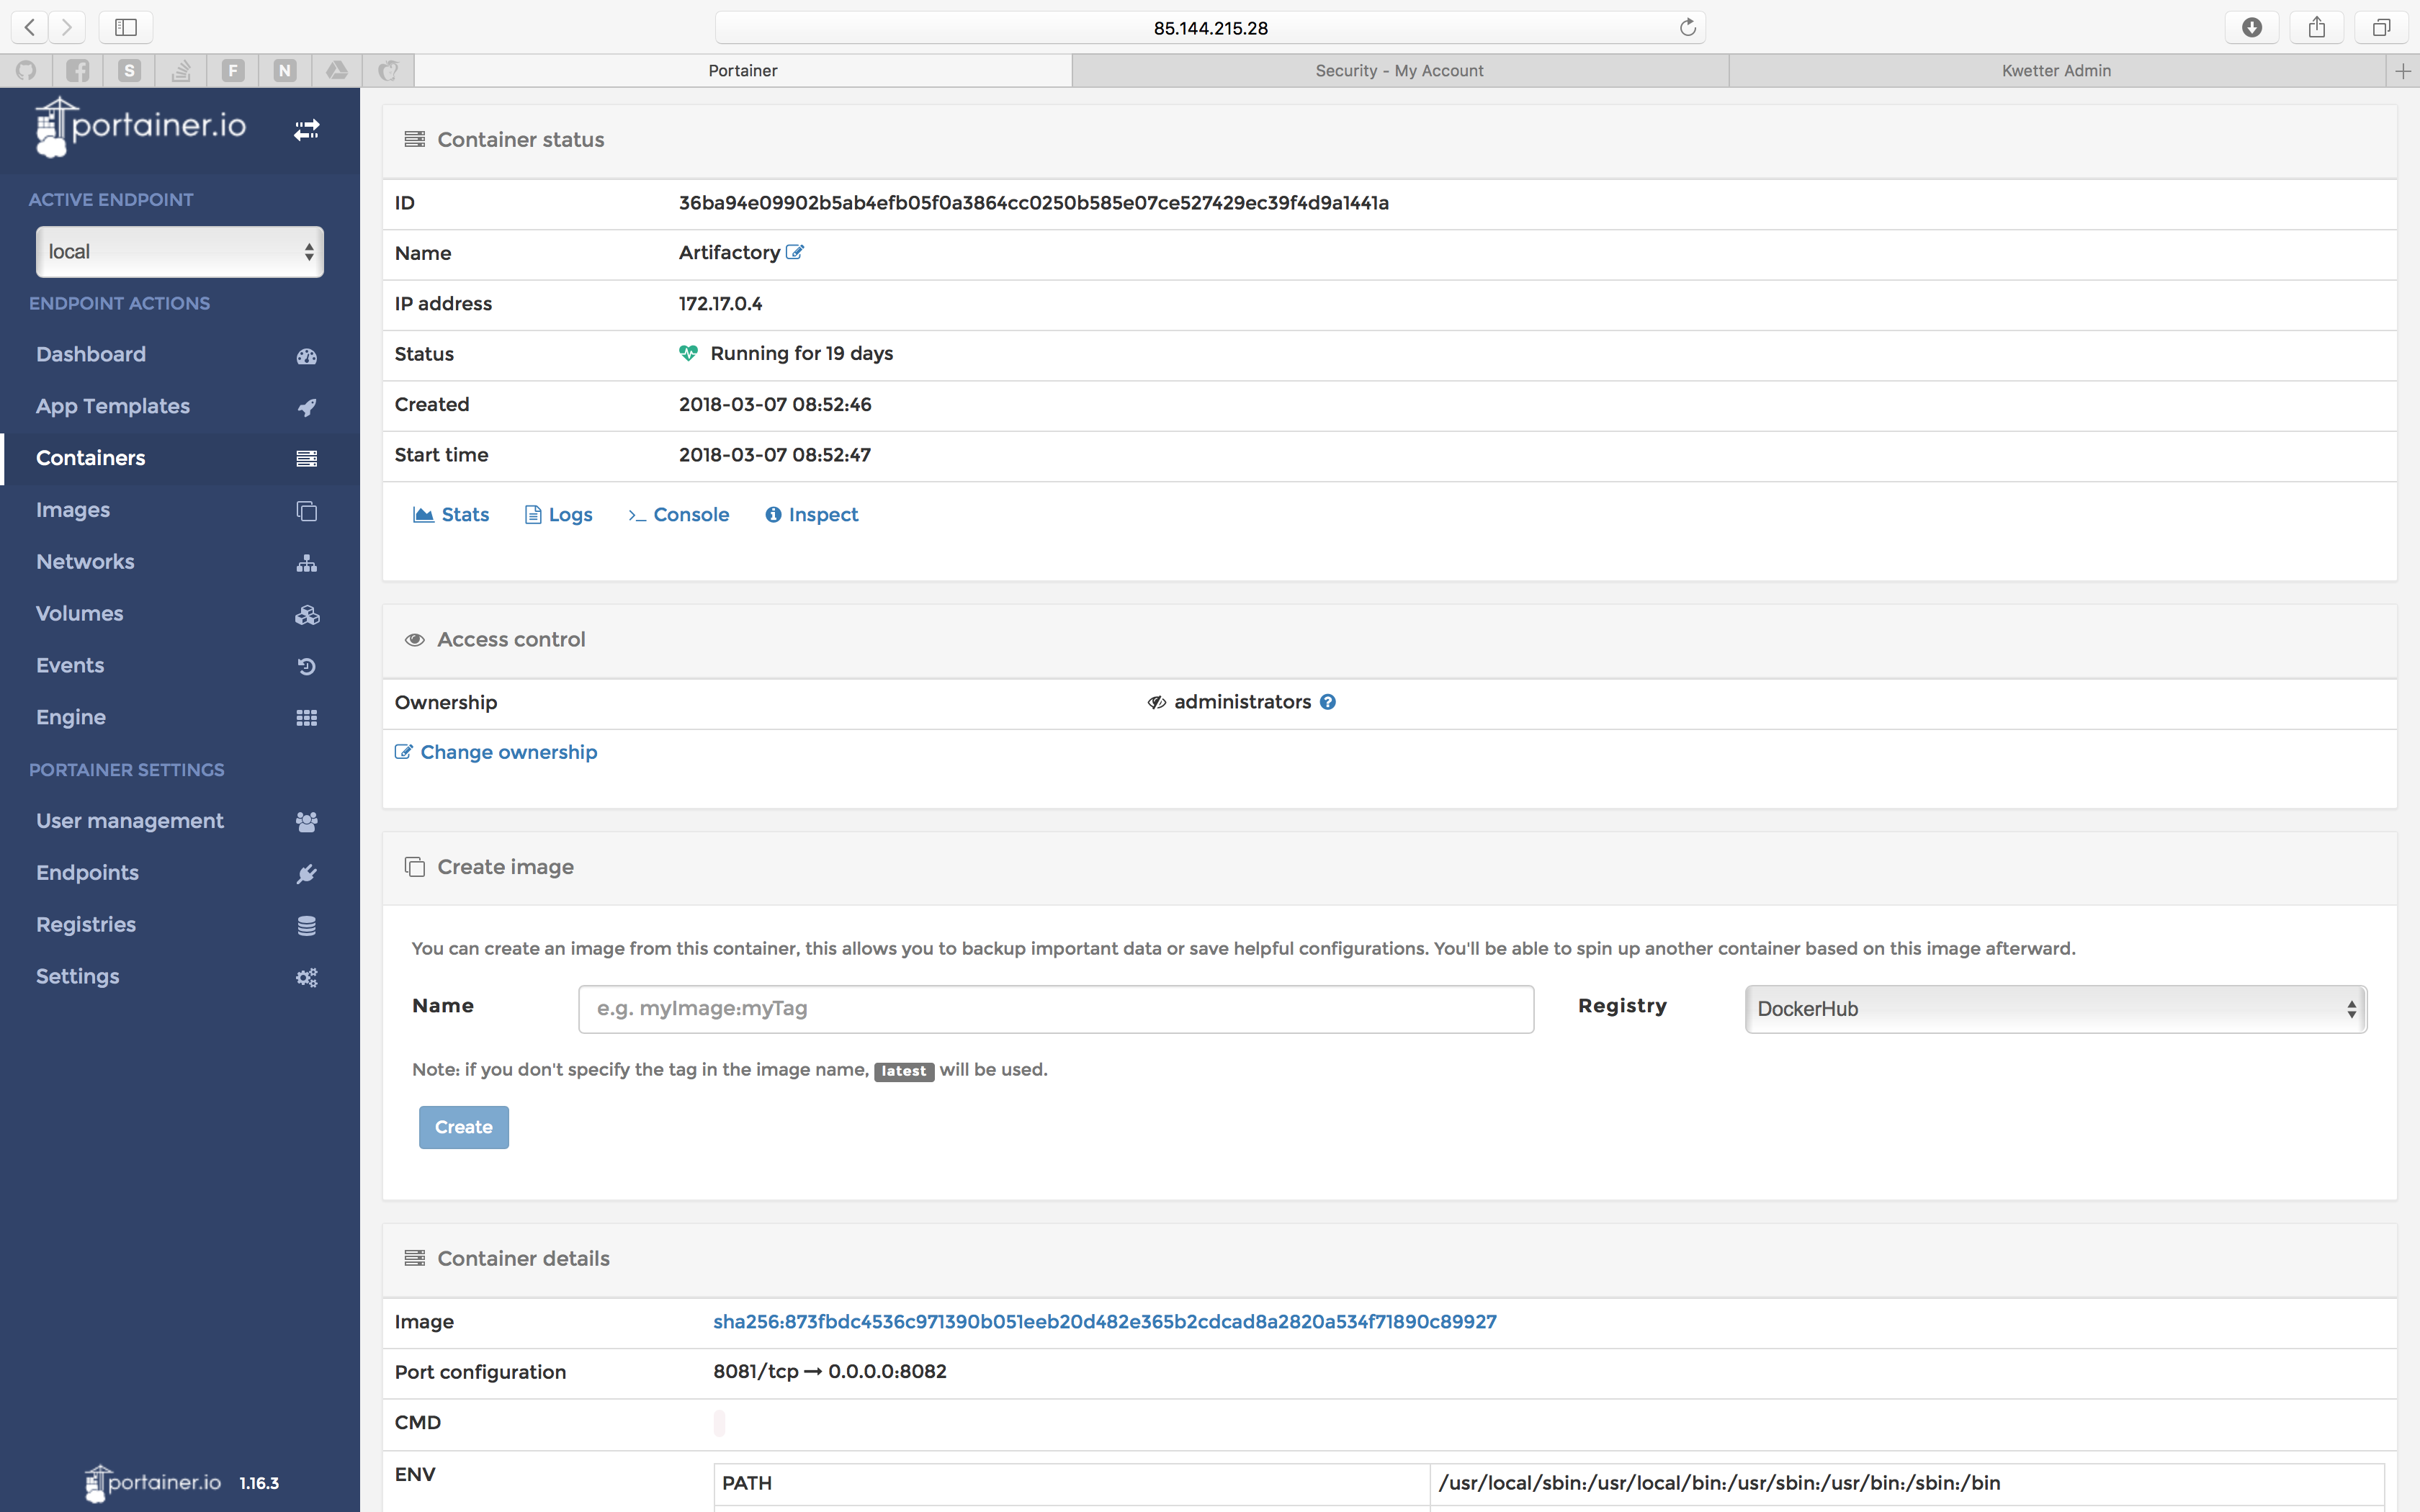
\includegraphics[width=0.95\textwidth]{img/ArtifactoryContainerDetails.png}
	\caption{Container configuratie voor Artifactory}
	\label{fig:ArtifactoryContainerDetails}
\end{figure}

\section{Configuratie van Artifactory}
Door middel van de Artifactory plugin in Jenkins kunnen we een .jar, .war, .ear, ... bestand automatisch deployen naar Artifactory. Hierdoor wordt de applicatie/dependency beschikbaar binnen de Artifactory repository. Om de gemaakte dependency binnen een project te kunnen gebruiken, is echter meer configuratie vereist op de lokale machine waar het programma wordt uitgevoerd.

\subsection{Configuratie van Artifactory in een Maven project}
Zoals aangegeven in hoofdstuk 3.2.1 Maven Settings, is het vereist om een aangepast configuratie aan te maken voor maven. In deze configuratie staan onder andere de inlog gegevens die vereist zijn om een verbinding met Artifactory op te zetten.
\newline
Voor elk project moeten we het configuratie bestand (pom.xml) aanpassen waardoor de connectie met Artifactory actief wordt. We hebben de configuratie van elk project aangepast waardoor de volgende onderdelen in de configuratie zijn opgenomen: 
\begin{itemize}
	\setlength\itemsep{0em}
	\item Distributie management
	\item repositories (lib-release en lib-snapshot die beschikbaar zijn vanuit Artifactory)
	\item plugin repositories (lib-release en lib-snapshot die beschikbaar zijn vanuit Artifactory)
\end{itemize}

\subsection{Library importen in een project vanuit Artifactory}
Wanneer de configuratie voor Artifactory in de lokale maven instellingen voor de verschillende servers (en tevens voor machines van ontwikkelaars) succesvol is uitgevoerd, is het mogelijk om libraries die beschikbaar zijn door middel van Artifactory te gebruiken in een of meerdere applicaties. Hiervoor moet in het configuratie bestand van de applicatie de juiste dependency worden toegevoegd.
\newline
In figuur \ref{fig:ArtifactoryDependencyManagement} is te zien welke versies van een library beschikbaar zijn in de repository. Wanneer we een versie van de library selecteren, krijgen we meer informatie te zien. Tevens staat er beschreven hoe we de library kunnen gebruiken bij een applicatie.

\begin{figure}[H]
	\centering
	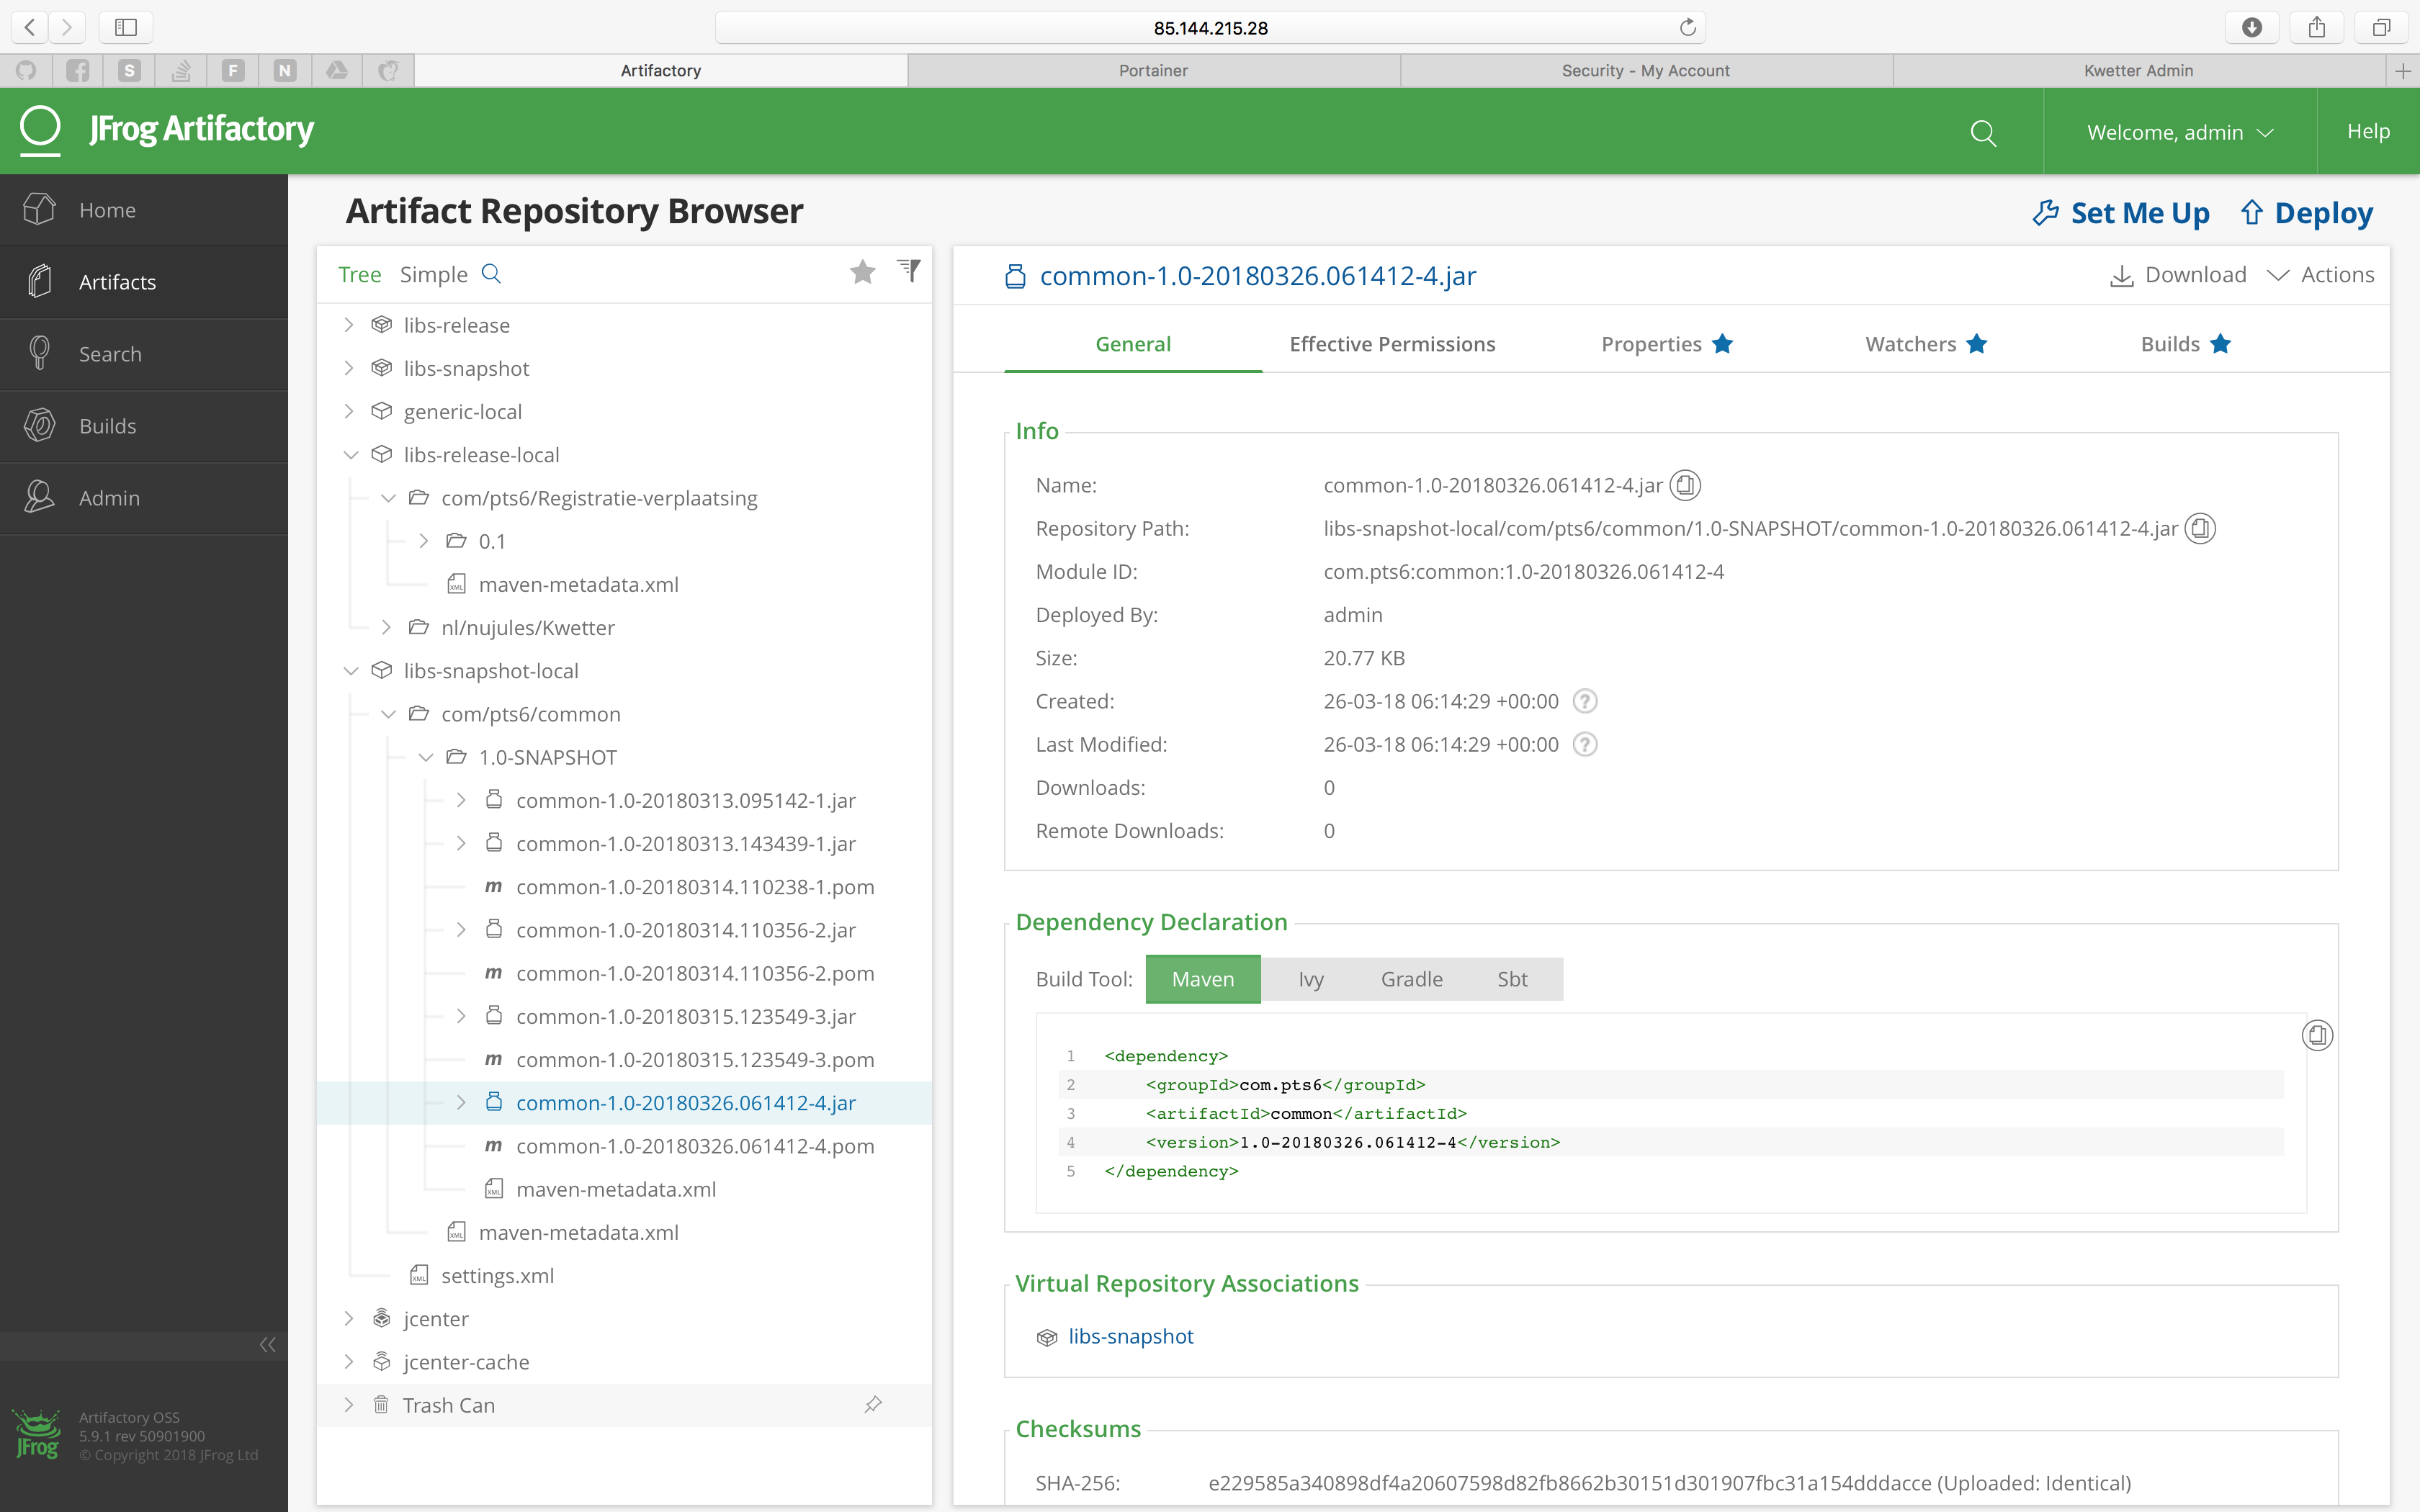
\includegraphics[width=0.95\textwidth]{img/ArtifactoryDependencyManagement.png}
	\caption{Artifactory library overzicht voor de "Common" library}
	\label{fig:ArtifactoryDependencyManagement}
\end{figure}